\chapter{Vincoli}
%\chapter{Constraints, Discoverability e Feedback}
\begin{flushleft}
	\textit{In che modo si riesce a capire una cosa che non abbiamo mai visto prima?}
\end{flushleft}

Non c'è altro da fare che combinare l'informazione presente nel mondo esterno con quella che si ha in testa.

L'insieme di conoscenze che si trovano nel mondo comprende le affordances, i significanti visibili, le corrispondenze fra quelle parti degli oggetti che sembrano comandi o punti da manipolare, le azioni risultanti e i vincoli fisici che limitano ciò che è possibile fare.

La conoscenza si ha in mente comprende i modelli concettuali, i vincoli culturali, semantici e logici del comportamento, le analogie fra la situazione attuale ed esperienze precedenti.

\begin{figure}[!h]
	\centering
	\includegraphics[scale = 0.7]{"immagini/Modellino Lego"}
	\caption{Un modellino lego.}
\end{figure}

Si prenda come esempio il modellino Lego presente in figura: ha 15 pezzi, solo alcuni specializzati, molti altri sono di grandezza e forma uguale ma di colori diversi. Combinando i vincoli fisici con quelli culturali, semantici e logici si riesce a costruire il modellino senza istruzioni, mettendo ogni pezzo nella sua giusta posizione.

Vincoli fisici limitano le parti che possono andare insieme, i vincoli culturali e semantici impongono restrizioni precise a tutti i pezzi restanti e se rimane fuori qualche pezzo l'incastro è dettato dalla logica.

\textbf{I vincoli sono indizi potenti}, che limitano l'insieme delle azioni possibili. L'uso intelligente dei vincoli in sede di design permette alle persone di decidere prontamente il giusto corso d'azione, anche in una situazione del tutto nuova.

\pagebreak

È possibile categorizzare i vincoli in \textbf{quattro} classi:
\begin{itemize}
	\item \textbf{Vincoli fisici}: si affidano a proprietà del mondo fisico, senza alcun bisogno di istruzioni o di addestramento. Nell'esempio della motocicletta Lego ritroviamo questo vincolo nei pezzi che si incastrano solo in un determinato verso.
	\item \textbf{Vincoli culturali}: si affidano alle abitudini culturali, sociali, comportamentali che possono cambiare nel tempo. Con \textbf{vincolo culturale} s'intendono anche le convenzioni. Nell'esempio della motocicletta Lego ritroviamo questo vincolo nel saper determinare la collocazione delle luci: bianco all'anteriore e rosso al posteriore.
	\item \textbf{Vincoli semantici}: si affidano al significato della situazione per circoscrivere l'insieme delle azioni possibili, si basano sulla conoscenza della situazione e del mondo. Nel caso della motocicletta, c'è un'unica collocazione sensata per il motociclista, deve stare seduto guardando in avanti.
	\item \textbf{Vincoli logici}: dettati dalla semplice e pura logica umana. Se avanzasse un un solo pezzo per assemblare la motocicletta, grazie alla logica sapremo dove collocarlo nella sua giusta posizione.
\end{itemize}

Un buon designer può sfruttare questi vincoli per veicolare l'utente verso un modello mentale del prodotto che si avvicini il più possibile al modello concettuale desiderato ed in tal modo garantirgli una UX gradevole.

%\section{Vincoli e mapping}
Vincoli e mapping a volte si confondono tra di loro. Una serie di interruttori mappati in maniera opportuna infondono un vincolo logico che permette all'utente di non sbagliare, si intuisce perfettamente cosa verrà azionato da quell'interruttore posto in quel determinato punto. \textbf{Mapping forti possono diventare dei vincoli logici}.
L'assenza di vincoli e mapping genera, come già ribadito più volte, frustrazione poiché crea una interfaccia poco chiara e difficile da comprendere.
\begin{figure}[!h]
	\centering
	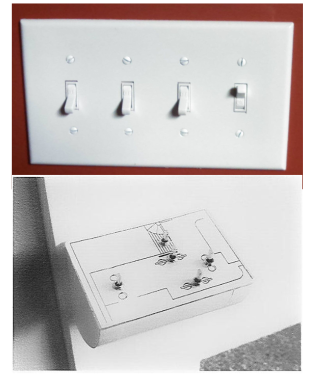
\includegraphics[scale=0.67]{immagini/Interruttori}
	\caption{Un interruttore per le luci di una stanza che imita la piantina del locale.}
\end{figure}

\pagebreak

\section{Funzioni Obbliganti}
\textbf{Le funzioni obbliganti sono una forma di vincolo fisico}: consistono di situazioni in cui le azioni sono vincolate in modo che un passaggio mancato impedisca di procedere al successivo.

Sono il caso estremo di vincoli atti ad impedire un comportamento inappropriato.

Non tutte le situazioni permettono l'uso di vincoli così forti, ma il principio generale è applicabile negli ambiti più diversi.

Si esaminano ora tre di questi metodi:
\begin{itemize}
	\item \textbf{Interlock}: obbliga a eseguire una serie di operazioni (n maggiore di 1) nella sequenza dovuta prima di avviare l'azione richiesta. Gli interlock sono usati soprattutto come sistemi di sicurezza nei macchinari idnustriali ma anche nel mondo software come per esempio nel caso dei sistemi Captcha.
	
	\begin{figure}[!h]
	\centering
	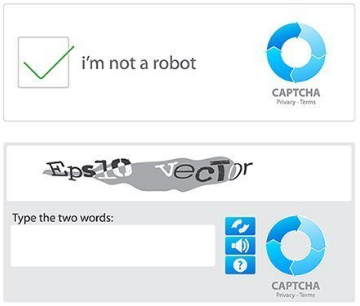
\includegraphics[width=0.4\textwidth]{immagini/cap.png}
	\caption{I captcha sono un esempio di interlocks.}
\end{figure}

\begin{figure}[!h]
	\centering
	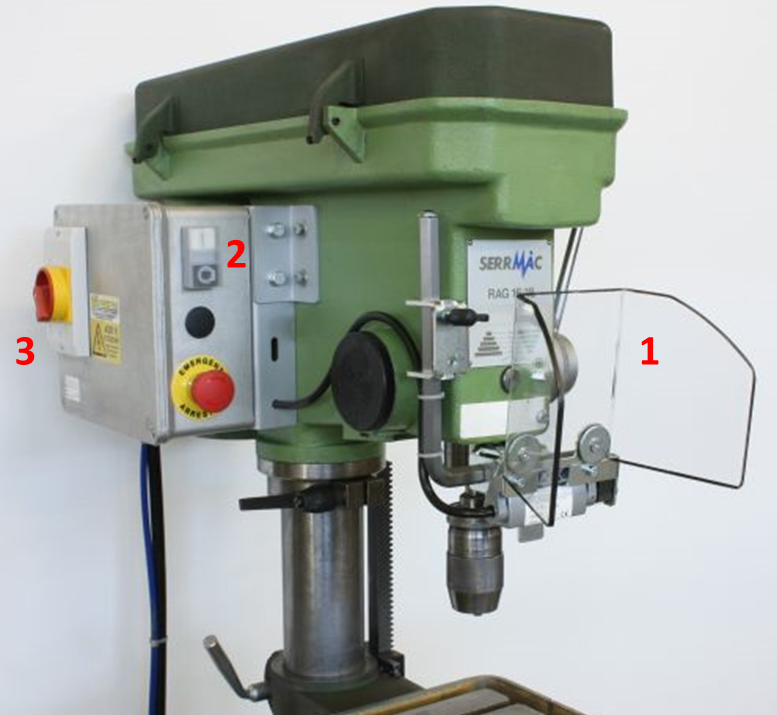
\includegraphics[width=0.5\textwidth]{immagini/trapano.png}
	\caption{Per usare un trapano a colonna professionale è necessario 1) chiudere lo sportello di sicurezza; 2) armare il sistema premendo l'apposito bottone; 3) attivare il motore ruotando l'interruttore rosso. Se uno di questi passaggi viene ignorato il sistema non si attiva. Se una volta attivato il sistema, lo sportello viene aperto il motore si spegne. }
\end{figure}

	\item \textbf{Lock-in}: mantiene attiva una funzione impedendo che qualcuno la interrompa prematuramente. È usato molto in ambito informatico (e.g. ogni tentativo di uscita da un'applicazione senza salvare è prevenuto da un messaggio di allerta che chiede la conferma dell'intenzione). \textbf{Per finire un task si deve compiere un'azione.}
	
	\begin{figure}[!h]
	\centering
	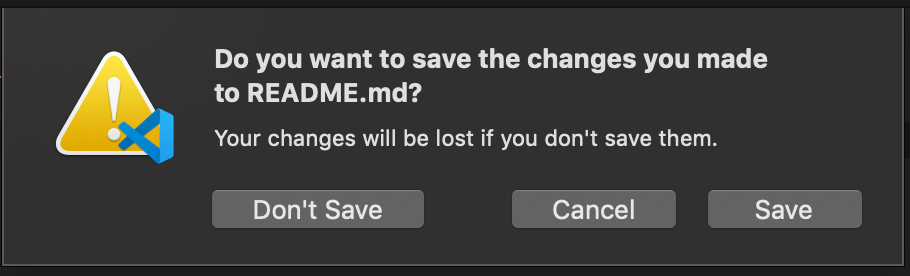
\includegraphics[width=0.4\textwidth]{immagini/savedialog.png}
	\caption{Il dialog dove viene proposto di salvare prima di chiudere è un esempio di lock-in dal momento che blocca "dentro" il software l'utente fino a che questo non da un ulteriore input.}
\end{figure}


	\item \textbf{Lockout}: impedisce l'ingresso in uno spazio pericoloso o impedisce che succeda qualcosa. Può essere considerato l'opposto del lock-in. Un esempio di stampo informatico, sono gli \textbf{alert VM 18} che si possono trovare su alcuni siti. \textbf{Per accedere ad un task si deve compiere un'azione.}
\end{itemize}

	\begin{figure}[!h]
	\centering
	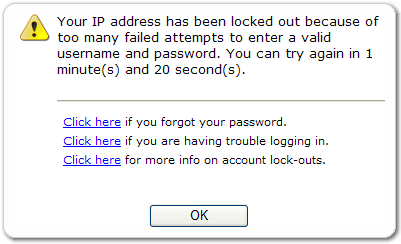
\includegraphics[width=0.5\textwidth]{immagini/lockout.png}
	\caption{Bloccare un utenza perchè ha immesso troppe volte credenziali sbagliate è un esempio di lock-out. Per superare il blocco bisogna attendere o seguire delle specifiche procedure.}
\end{figure}



\section{Activity-Centered Control}
Il mapping spaziale dei comandi non sempre è il più opportuno.

In molti casi è meglio avere interruttori diversi per attività diverse: \textbf{comandi centrati sulle attività}.

Azionando un semplice comando si impostano una serie di oggetti per svolgere una determinata attività, senza comandarli uno ad uno. In molti auditorium ci sono interruttori con indicazioni \textit{video}, \textit{computer}, \textit{piena luce} e \textit{lezione} che impostano il microfono, le luci della sala, il proiettore e quant'altro.

Questo schema è eccellente in teoria, ma nella pratica è difficile da realizzare bene, soprattutto è necessario valutare gli \textbf{imprevisti} e le possibili risoluzioni.

Per carità, il metodo è giusto, purché la gamma di attività sia scelta in modo da corrispondere alle situazioni reali. Ma anche in quel caso saranno pur necessari dei comandi manuali, perché si presenteranno sempre esigenze inattese, che richiederanno una regolazione particolare dei dispositivi.

La Logitech ha prodotto una serie di telecomandi universali completamente progettati attorno al concetto degli Activity Centereed Control \url{https://www.logitech.com/it-it/harmony-universal-remotes}.

	\begin{figure}[!h]
	\centering
	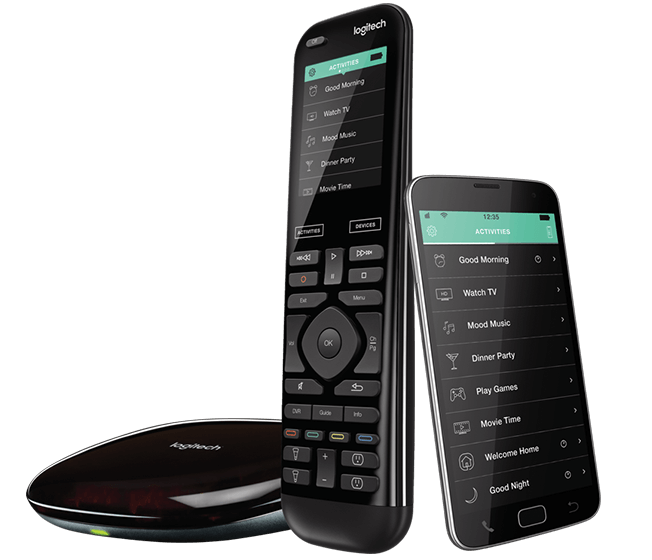
\includegraphics[width=0.5\textwidth]{immagini/harmony.png}
	\caption{Il telecomando universale Harmony di Logitech consente di controllare vari dispositivi attraverso un modello di interazione basato sugli activity centered controls. Non si seleziona più il dispositivo che si vuol controllare ma l'attività che si vuol fare: Play Game, Watch TV, etc..}
\end{figure}
